\chapter{Organizacion}

\section{Introdución}

La generación de residuos sólidos a nivel mundial es directamente proporcional a la explosión demográfica y al crecimiento económico, se trata de un fenómeno natural asociado a los asentamientos humanos, que en las últimas cinco décadas ha resultado en una explotación descontrolada de todo tipo de recursos naturales debido a la industrialización, urbanización y cambio en el estilo de vida, lo que ha generado el aumento de residuos en cuanto a cantidad y complejidad.

En el presente siglo, el calentamiento global genera preocupación generalizada por la contaminación y sus efectos medioambientales en el planeta, desde entonces se han generado políticas y planes para el manejo adecuado de basuras. En Colombia hay varios sistemas de disposición final para los residuos sólidos entre los cuales están; enterramientos, plantas integrales, botaderos, quemas, cuerpos de agua y rellenos sanitarios, siendo este último el más usado en el país, para Bogotá estas políticas están enfocados parcialmente en la educación del habitante, en la disposición de puntos de recolección especializados y en la concientización de la necesidad de tener hábitos amigables con el medio ambiente según lo describe el programa basura cero de la capital que funciono desde el año 2012 al 2016.

Es así como la investigación elaborada, propone el desarrollo de un prototipo la cual contará con varios módulos, que le permitirá al usuario obtener información detallada del proceso que sufrirá los residuos no orgánicos reciclables que quiere poner a disposición de los centros de reciclaje, este proceso lo completan los operarios del reciclaje los cuales irán a recoger estos residuos y enviarlos al centro más cercano este proceso permitirá saber dónde y cómo se debe desechar estos elementos, además de poder gestionar y tener un  histórico de  los  recursos  reciclables.

En el presente documento se describe un problema, tomándolo como punto de partida para el análisis, desarrollo e implementación del proyecto. Para tal efecto se aplicará la metodología RUP para documentar y desarrollar las fases del proyecto; entre esas se encuentra la fase de análisis donde se plantea y se define la solución más óptima para gestión de residuos no orgánicos reciclables, y a partir de estas se empieza una construcción de varios prototipos en la fase de diseño, en la que se construyen los modelos del lenguaje de modelado visual UML donde se termina con la etapa de implementación y pruebas.  

También muestra el posible uso de las aplicaciones distribuidas, que ayuda al mejoramiento de los procesos previamente descritos, mediante un conjunto de módulos, un portal web, web api y aplicación móvil logrando así dar una idea sobre como el uso de las tecnologías de la información pueden ayudar a solucionar un problema medioambiental.


\section{Nombre}

Chatarrapp


\subsection{Misión}

Concientizar y educar a la sociedad sobre la importancia de la preservación del medio ambiente, bajó su participación activa en la realización y ejecución del proyecto Chatarrapp que surjan desde un pensamiento ecológico y sustentable, sugiriendo respuestas inmediatas a situaciones que afecten el medio ambiente.


\subsection{Visión}

Ser la primera organización que establece una arraigada cultura ecológica, por la calidad, confiabilidad, conocimientos, y servicios que cumpliran las necesidades de las tecnologías de la comunicación en Colombia enfocadas a la mejora del medio ambiente, lográndolo a través de un trabajo en equipo comprometido, con una planificación y organización adecuada, y que  construya una conciencia ambientalista.


\newpage

\subsection{Objetivos}

Desarrollar un prototipo multiplataforma para que los ciudadanos y centros de  reciclaje gestionen la recolección de elementos no renovables reciclables con el fin de promover el cuidado del medio ambiente en la localidad de Usme


\subsection{Organigrama}

\begin{figure}[h!]
	\centering
	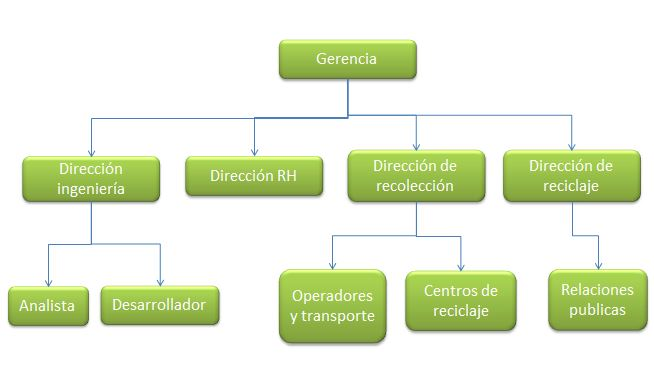
\includegraphics[width=0.7\linewidth]{Proyecto/Organizacion/imgs/Organigrma}
	\caption{Cronograga}
\end{figure}


\subsection{Funciones}

\title{Analista de sistema}
El analista de sistemas evalúa de manera sistemática el funcionamiento, mediante el examen de la entrada y el procesamiento, con el propósito de mejorar los procesos de una organización. 
Rol de consultor del analista de sistemas
Rol de experto en soporte tecnico del analista de sistemas
Rol de agente de cambio del analista de sistemas

\title{Desarrollador de Software}
su principal responsabilidad es definir y mantener el código fuente de uno o varios componentes, garantizando que cada componente implemente la funcionalidad correcta.
Rol de integridad de uno o más subsistemas de implementación y de sus contenidos a lo largo del desarrollo. 
Rol de asegurar el código libre de errores y pruebas unitarias del código construido.

\title{Operadores y Transporte}
Se encarga de los aspectos logísticos, ademas de todos los procesos de la cadena de suministro, proceso de pedidos, almacenamiento, empaque, transporte.

\title{Centro de reciclaje}
Empresa que realiza el oficio de recolectar, seleccionar, recuperar, transformar, comercializar y reutilizar los residuos sólidos. Cumple la labor de reciclar en el primer eslabón de la cadena de comercialización y recuperación de material.

\title{Relaciones publicas}
responsable de la creación de un concepto de sistema que ayude a cumplir los objetivos de negocio fijados por los interesados, asegurándose que el sitio cumpla con las características de accesibilidad, navegabilidad, interactividad y usabilidad que garanticen una experiencia agradable al usuario. 


\subsection{Prodcuto}

5820 Edición de programas de informática (software)
6201 Actividades de desarrollo de sistemas informáticos (planificación, análisis, diseño, programación, pruebas)
6209 Otras actividades de tecnologías de información y actividades de servicios informáticos
